\section[Problem 5]{Problem 5: Depot Activation and Relief Allocation on the Flood-Cut Network}
\label{sec:q5}

\subsection{Task, Decision Time and Demand}

Among the tasks offered by the problem we choose emergency supply allocation combined with the choice of which relief depots to open: on a given day, which of the candidate depots should be activated, and how many tonnes of daily relief kits should each open depot send to each affected settlement catchment over the road network that is still passable. The main decision time is $T_0=16$ July 2026, the moment the Sentinel-1 pass of that day has been processed. As a second decision time we use 4 July, to measure what the later pass is worth.

Demand comes directly from Problem~4. With the flooded population $P_j$ of unit $j$ and the relief need of Assumption~6,
\begin{equation}
d_j=\frac{q\,H\,P_j}{1000}\ \ [\mathrm t],\qquad q=3.5\ \mathrm{kg\,person^{-1}\,day^{-1}},\quad H=3\ \mathrm d,
\label{eq:demand}
\end{equation}
and the priority of the unit is its disaster index, $w_j=\max(S_j,0.001)$. The floor keeps the lowest-ranked affected unit in the objective. Affected units with at least one flooded person form 164 demand units with a total demand of 146.46\,t.

\subsection{Flood-Cut Network and Admissible Assignments}

OSM roads are snapped at 1\,m into a directed graph (one-way tags respected) with edge time equal to length over a class speed reduced for emergency driving (80\,km/h on motorways down to 15\,km/h on tracks). Every edge that touches the 16 July raster $F$ under the 20\,m buffer rule is deleted. 117.4\,km of road disappear. The flooded-population centroid of each unit is connected to the nearest node of the cut graph by an access leg of at most 5\,km at 15\,km/h. Candidate depots are the 16 town nodes, the city node and the schools, merged within 300\,m to 21 candidates. A candidate is excluded if it lies within 100\,m of $F$ or more than 1\,km from the cut graph, which leaves 20. The travel time $t_{ij}$ is the depot access time plus the Dijkstra time on the cut graph plus the demand access time, infinite if no path exists, and the admissible pairs are
\begin{equation}
\mathcal A=\{(i,j):\ t_{ij}\le T_{max}\},\qquad T_{max}=120\ \mathrm{min}.
\label{eq:admissible}
\end{equation}
This gives 1189 admissible pairs. For 57 demand units no candidate is admissible: the flood has cut every road path to them within two hours. In this way the image result enters the optimization twice, through the deleted roads and depots and through $d_j$ and $w_j$.

\subsection{A Bi-objective Location--Allocation MILP}

\textbf{Decision variables.} Opening a depot is a yes-or-no decision, so the depot variable is binary:
\begin{equation}
\eta_i=\begin{cases}1, & \text{candidate depot } i \text{ is activated on the decision day},\\ 0, & \text{otherwise},\end{cases}\qquad i\in\mathcal I,\ |\mathcal I|=20 .
\label{eq:eta}
\end{equation}
The shipment $x_{ij}\ge0$ (tonnes from depot $i$ to unit $j$, defined only for $(i,j)\in\mathcal A$) and the unmet demand $u_j\ge0$ are continuous, because relief kits are counted in thousands and their tonnage is effectively divisible.

\textbf{Objectives.} Resources are limited, so relief has to serve ``areas and populations in urgent need of assistance in a more timely and targeted manner''. ``Targeted'' is measured by the priority-weighted unmet share and ``timely'' by the priority-weighted delivery time, both minimized:
\begin{equation}
\min\ f_1=\frac{\sum_jw_ju_j}{\sum_jw_jd_j},\qquad
\min\ f_2=\frac{\sum_{(i,j)\in\mathcal A}w_j\,t_{ij}\,x_{ij}}{\sum_jw_jd_j}\ \ [\mathrm{min}].
\label{eq:q5_obj}
\end{equation}
Both are normalized by the same weighted demand, so $f_1\in[0,1]$ and $f_2$ is an average delivery time in minutes per weighted tonne.

\textbf{Constraints.}
\begin{equation}
\begin{aligned}
\text{s.t.}\quad
&\sum_{i:(i,j)\in\mathcal A}x_{ij}+u_j=d_j, && \forall j,\\
&\sum_{j:(i,j)\in\mathcal A}x_{ij}\le C_i\,\eta_i, && \forall i\in\mathcal I,\\
&x_{ij}\le d_j\,\eta_i, && \forall (i,j)\in\mathcal A,\\
&\sum_{i\in\mathcal I}\eta_i\le K,\\
&\sum_{(i,j)\in\mathcal A}\frac{2t_{ij}+t_l}{Q_v}\,x_{ij}\le 60\,N_vT_sH,\\
&x_{ij}\ge0,\quad u_j\ge0,\quad \eta_i\in\{0,1\}.
\end{aligned}
\label{eq:q5_cons}
\end{equation}
Each unit's demand is balanced between deliveries and unmet need, and no shortfall can hide. Tonnage is capped at the depot's horizon capacity ($C_i=60$\,t for a town or school, 200\,t for the city) and, through $\eta_i$, only open depots may ship; this is the standard linear form of a fixed opening decision, $C_i$ being the tightest valid bound; no artificial constant is needed. The linking bound $x_{ij}\le d_j\,\eta_i$ is redundant for integer solutions and tightens the LP relaxation, since no unit can receive more than its demand from one depot. Staff and stock for more than $K=6$ sites are not available. What remains is the fleet budget: a round trip of $2t_{ij}$ plus $t_l=30$\,min for loading carries $Q_v=5$\,t, and $N_v=40$ trucks working $T_s=12$\,h per day over $H=3$ days provide $60N_vT_sH=86{,}400$ vehicle-minutes. Aggregate vehicle-minutes, not a routing model; the time limit enters through $\mathcal A$.

\textbf{Model class and solution method.} The model is a mixed-integer linear program with 20 free binary variables (the excluded candidate is fixed closed) and 1353 continuous variables (1189 shipments, 164 unmet demands), and 1375 structural constraints (164 balances, 20 capacities, 1189 linking bounds, one depot limit, one fleet budget). With only 20 binaries an exact branch-and-bound solve is cheap; no heuristic is needed. We use the HiGHS solver~\cite{huangfu2018highs} with relative gap 0. The recommended plan is lexicographic, because covering need is more important than speed: stage 1 computes $f_1^*=\min f_1$ subject to \eqref{eq:q5_cons}, stage 2 minimizes $f_2$ subject to \eqref{eq:q5_cons} and $f_1\le f_1^*+10^{-6}$. The trade-off is then traced by the $\varepsilon$-constraint method, $\min f_2$ subject to $f_1\le\varepsilon_k$ with $\varepsilon_k=f_1^*+\frac{k}{14}(1-f_1^*)$ for $k=0,\dots,14$, and the knee is the front point farthest from the chord between its end points on normalized axes. Every solve returned status optimal with zero gap.

\subsection{Recommended Relief Plan for 16 July}

The lexicographic solve opens six depots. Table~\ref{tab:q5_plan} lists them with their shipments.

\begin{table}[H]
\centering
\caption{Open depots of the recommended plan}
\label{tab:q5_plan}
{\small\renewcommand{\arraystretch}{0.86}
\begin{tabularx}{\dimexpr\linewidth-4.6pt\relax}{l*{3}{>{\centering\arraybackslash}X}}
\toprule
Depot & Type & Capacity (t) & Shipped (t) \\
\midrule
Taoxu & town & 60 & 39.59 \\
Yunbiao & town & 60 & 28.82 \\
Shitang & town & 60 & 5.65 \\
Gaocun & school & 60 & 1.97 \\
Zhenlong & town & 60 & 0.66 \\
Liujing & town & 60 & 0.13 \\
\midrule
Total & & 360 & 76.82 \\
\bottomrule
\end{tabularx}}
\end{table}

The plan reaches $f_1^*=0.570$ and $f_2=13.05$\,min. It ships 76.82 of the 146.46\,t demanded and serves 7316 of the 13,948 people in the demand units. Fig.~\ref{fig:q5_route_alloc} draws the delivery paths on the cut network.

\begin{figure}[H]
  \centering
  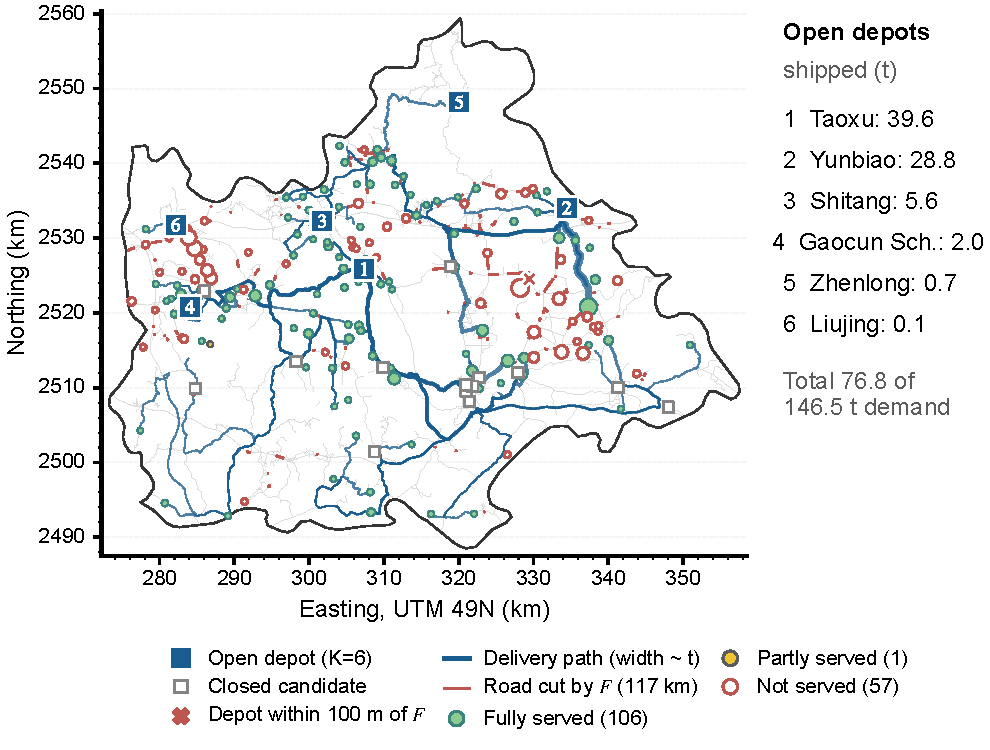
\includegraphics[width=0.98\textwidth,keepaspectratio]{../figures/fig_q5_route_alloc.pdf}
  \caption{Recommended relief plan}
  \label{fig:q5_route_alloc}
\end{figure}

Taoxu and Yunbiao, the two largest depots, supply 89\% of the tonnage through short paths into the central and eastern flood belt; Shitang and the Gaocun school serve the north and west; Zhenlong and Liujing cover small remote demands. More than half of the weighted demand stays unmet even though the open depots hold 360\,t, almost 2.5 times the total demand, and the fleet uses 1497 of 86,400 vehicle-minutes. Capacity is not the bottleneck, and neither are trucks. Reachability is. Water cuts off the 57 units that have no admissible depot, and no allocation over the road network can reach them. To six decimals the optimum equals the weighted demand of those 57 units (0.569927, against $f_1^*=0.569928$); the allocation carries no slack, every reachable unit is served in full, and no shipment on this network can lower $f_1$. Operationally this is the finding that matters, and it is why the letter asks for boats and helicopters for these units.

\begin{table}[H]
\centering
\caption{The flood map as an input to the relief plan}
\label{tab:q5_nomap}
{\small\renewcommand{\arraystretch}{0.86}
\begin{tabularx}{\dimexpr\linewidth-4.6pt\relax}{l*{3}{>{\centering\arraybackslash}X}}
\toprule
Plan & $f_1$ & $f_2$ (min) & Served \\
\midrule
MILP on 16 July (recommended) & 0.570 & 13.05 & 7316 \\
Same model, flood map withheld & 0.001 & 14.55 & 13924 \\
\quad replayed on the real cut network & 0.592 & 20.52 & 6997 \\
Greedy nearest-depot & 0.573 & 9.47 & 7237 \\
Proportional to depot capacity & 0.570 & 19.55 & 7316 \\
\bottomrule
\end{tabularx}}
\end{table}

Table~\ref{tab:q5_nomap} prices the flood map itself. Withheld from the model, the same objective reports a nearly perfect plan: $f_1=0.001$, 13,924 people served. Replayed on the network the water actually cut, that plan serves 6,997 people at $f_1=0.592$ -- 318 fewer than the plan that saw the map -- and takes 20.52\,min against 13.05. The map is not a refinement of the answer; it is what makes the answer feasible. Two heuristics bound that point from below. A greedy nearest-depot rule gives up 0.3 points of coverage for 3.6\,min of speed; splitting tonnage in proportion to depot capacity reproduces the optimal coverage exactly and takes 6.5\,min longer.

\subsection{Trade-off, Value of Information and Sensitivity}

Two questions remain: whether the recommended plan is a reasonable compromise between coverage and speed, and whether a later satellite pass changes it. Fig.~\ref{fig:q5_pareto} addresses both with the $\varepsilon$-constraint front and 30 one-at-a-time exact re-solves.

\begin{figure}[H]
  \centering
  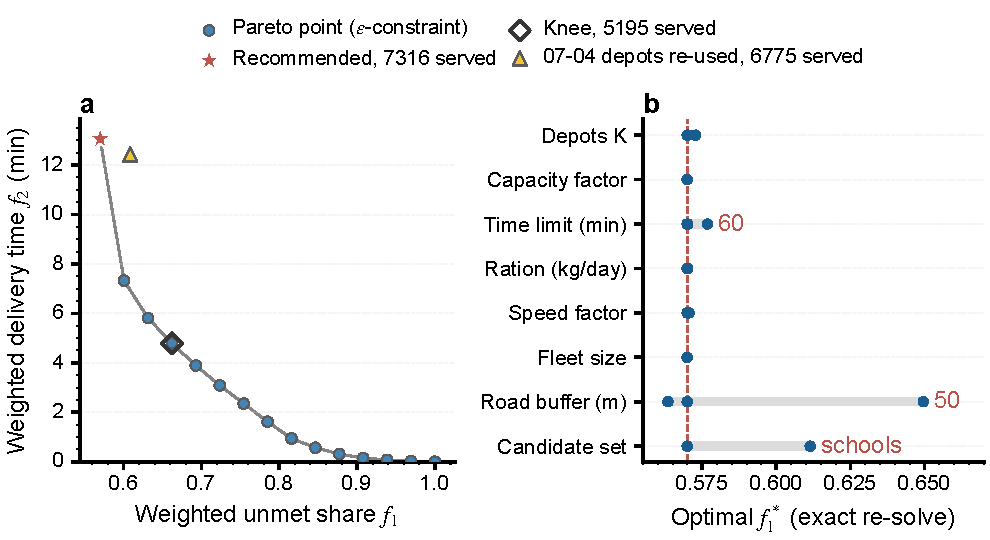
\includegraphics[width=0.98\textwidth,keepaspectratio]{../figures/fig_q5_pareto.pdf}
  \caption{Pareto front and sensitivity of $f_1^*$}
  \label{fig:q5_pareto}
\end{figure}

The front in panel (a) runs from the recommended plan $(f_1,f_2)=(0.570,13.05\ \mathrm{min})$ with 7316 people served to $(1,0)$ with nothing delivered. Its knee lies at $k=3$ with $f_1=0.662$, $f_2=4.79$\,min and 5195 people served: accepting 9 percentage points more unmet need would cut the average delivery time by 63\%. Because the problem stresses serving people in urgent need, we keep the coverage-first plan and report the knee as the alternative if speed matters more, for example for medical supplies.

Measuring the information update takes two solves. Built on the 4 July inputs, the plan opens Xiaoyi, Yunbiao, Liujing, Zhenlong, Hengzhou Town and the Gaocun school, and reaches $f_1=0.477$ under its own inputs. Keeping those depots but re-optimizing shipments against the 16 July cut network and demand gives $f_1=0.609$, $f_2=12.43$\,min and 6775 people served. The value of information is
\begin{equation}
\begin{split}
\mathrm{VoI}_1&=f_1^{04\to16}-f_1^{*,16}=0.609-0.570=0.039,\\
\mathrm{VoI}_2&=f_2^{04\to16}-f_2^{16}\big|_{f_1\le0.609}=12.43-6.89=5.54\ \mathrm{min},
\end{split}
\label{eq:voi}
\end{equation}
i.e. re-planning with the 16 July image lowers the weighted unmet share by 3.9 points, or, at equal coverage, delivers 5.54\,min faster. Read as a two-stage decision, 4 July is the first stage and the 16 July pass is the recourse a real operation would run. A frozen plan then loses at least 3.9 points and 5.5\,min: keeping the first-stage depots and re-optimizing only the shipments already leaves 0.609, the best a stale depot set can do. The tail sits in the depot set itself. Between the two dates the open sets share only half their members (Jaccard 0.50), total demand changes by $-3.57$\,t, and 677 admissible pairs are lost while 625 are gained, because the flood moved. That is the quantity the next satellite pass is worth.

Inputs can also be moved under a frozen plan. Six depots stay fixed and only the shipments are re-optimized -- the recourse an operation would actually run -- while 600 scenarios perturb the demand and the network (Table~\ref{tab:q5_cvar}, Fig.~\ref{fig:q5_cvar}). Demand noise of 20\% (lognormal, truncated at three sigma) moves $f_1$ by nothing, because geometry, not the size of the demand, is the binding constraint. Network noise does cost: cutting each of the 625 pairs that only reopened after 4 July with probability 0.5 gives $f_1=0.604$ and a 5\% quantile of 6345 people served. Over all 600 scenarios $\mathrm{CVaR}_{95}=0.651$; the plan reads as a promise that in 95\% of the futures consistent with the two passes it loses at most eight points of coverage, and in 63\% of them it stays below 0.60. Every reopened pair cut again, the stress case, serves 5846 people at $f_1=0.670$: 20\% fewer than the point estimate, the price of that many roads closing, and the plan never becomes infeasible.

\begin{figure}[H]
  \centering
  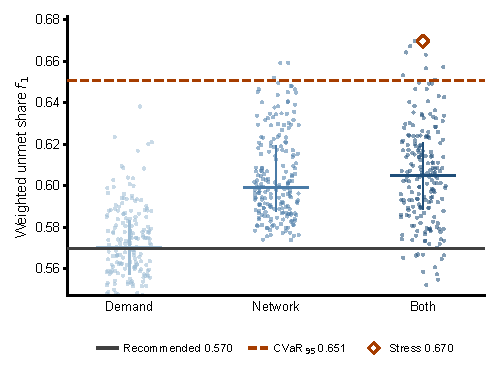
\includegraphics[width=0.86\textwidth,keepaspectratio]{../figures/fig_q5_cvar.pdf}
  \caption{Frozen-plan coverage under 600 scenarios}
  \label{fig:q5_cvar}
\end{figure}

\begin{table}[H]
\centering
\caption{Frozen plan under demand and network uncertainty, 600 scenarios}
\label{tab:q5_cvar}
\small
\begin{tabular}{lrrrr}
\toprule
Scenario family & $f_1$ mean & $f_1$ CVaR$_{95}$ & Served mean & Served $p_{05}$ \\
\midrule
Demand, $\sigma=0.2$ & 0.570 & 0.615 & 7316 & 7316 \\
Network, half of the reopened pairs cut & 0.604 & 0.650 & 6787 & 6345 \\
Both & 0.605 & 0.658 & 6795 & 6468 \\
\midrule
All 600 & 0.593 & 0.651 & 6966 & 6468 \\
Stress, every reopened pair cut & 0.670 & -- & 5846 & -- \\
\bottomrule
\end{tabular}
\end{table}

Panel (b) shows how $f_1^*$ responds to the assumed resources. It is non-increasing in the depot limit, from 0.5728 at $K=3$ to 0.5699 at $K=8$, while the delivery time drops from about 22\,min for $K\le5$ to 9.32\,min at $K=8$. Halving or raising capacity by 50\% leaves $f_1^*=0.5699$; the time limit changes it only at 60\,min (0.5768); the relief norm from 2.5 to 15.6\,kg per person and day changes it by less than 0.0003; a speed factor of 0.6 gives 0.5705, and the fleet size (20, 40 or 60 trucks) has no effect. Only two settings move $f_1^*$ by more than 0.005. The road buffer does: without a buffer $f_1^*=0.564$, with a 50\,m buffer 0.650, because more roads are cut. Restricting the facility proxies to schools alone gives four open depots, $f_1^*=0.611$ and $f_2=21.08$\,min. The plan is therefore robust to the logistic parameters we had to assume and sensitive to the flood extent on the roads, which is the quantity the remote-sensing chain measures.

The allocation is also checked for equity. For every demand unit with at least one admissible pair, a floor $\sum_i x_{ij}\ge q\,d_j$ is added and $q$ scanned from 0 to 1 in steps of 0.2. At the base budget---six depots, 360\,t of capacity against 146.46\,t of demand---nothing moves: $f_1=0.570$, $f_2=13.05$, the reachable unmet share stays zero at every $q$, and the same six depots open. For the 57 units that carry the whole shortfall no admissible pair exists; their gap is geographic, and no allocation rule closes it. Equity here is bounded by geography, not by the objective. The floor binds only when the depot budget is cut: at $K=3$ the base plan already leaves 0.29\% of reachable demand unmet ($f_1=0.573$, $f_2=22.24$, 7237 served) and $q=0.2$ is infeasible. What limits the service floor is therefore the number of staffed sites, not the tonnage: 360\,t covers 146.46\,t with slack, while three depots cannot span the 120-minute catchment. A policy that raises the floor has to add sites, not supplies.

All 19 saved plans (recommended, 4 July, recourse, knee and the 15 front points) were rechecked from the raw inputs with freshly computed shortest paths. Every demand balance closes to within $10^{-6}$\,t, no depot ships more than its capacity or while closed, no plan opens more than six depots, every positive shipment runs on a path within 120\,min that avoids $F$, no open depot lies within 100\,m of new inundation, and the recomputed demands equal the Problem~4 values\cite{deepseek2026,qwen2026,doubao2026}.
